\subsection {Patched TIMELY}
\label{sec:timely_fixed}
%\begin{figure}[t]
%\center
%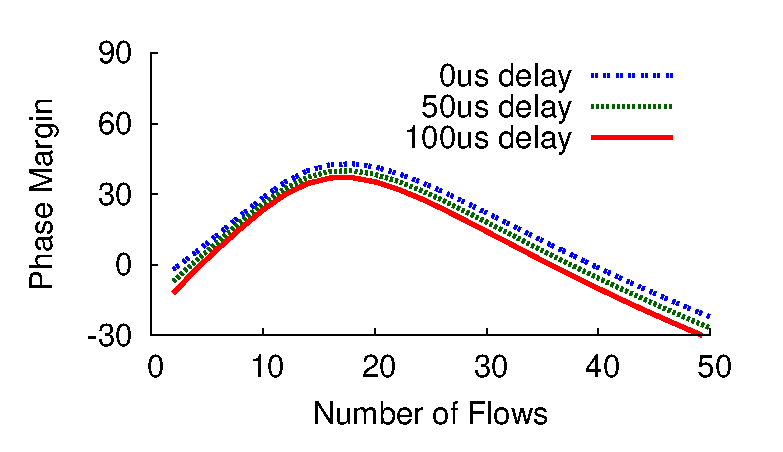
\includegraphics[width=0.33\textwidth]{figures/timely_stability.eps}
%\caption{Patched TIMELY stability}
%\label{fig:timely_stability}
%\end{figure}

\begin{figure*}[t]
\center
\subfigure[Two flows, 7Gbps and 3Gbps] { 
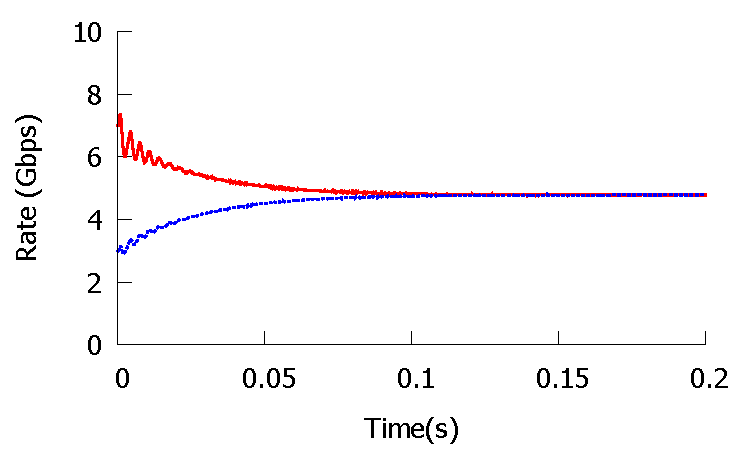
\includegraphics[width=0.3\textwidth]{figures/timely_stability_2f73_fixed.pdf}
\label{fig:timely_fixed_a}
}
\subfigure[Two flows, 7Gbps and 3Gbps] { 
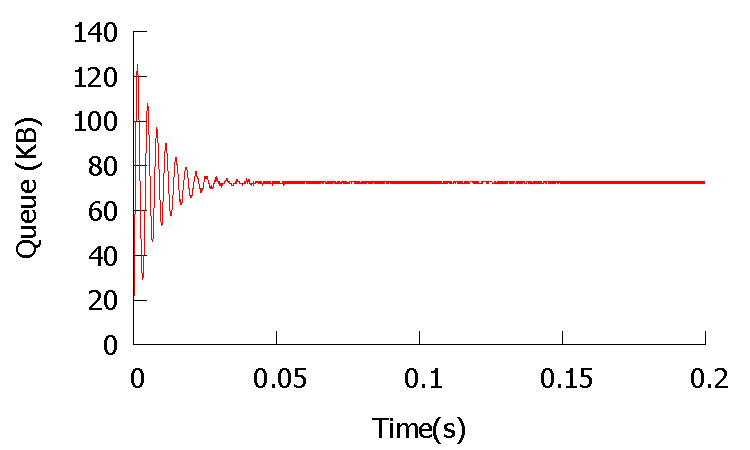
\includegraphics[width=0.3\textwidth]{figures/timely_stability_q_2f73_fixed.pdf}
\label{fig:timely_fixed_b}
}
\subfigure[40 flows, starting at 0.25Gbps] { 
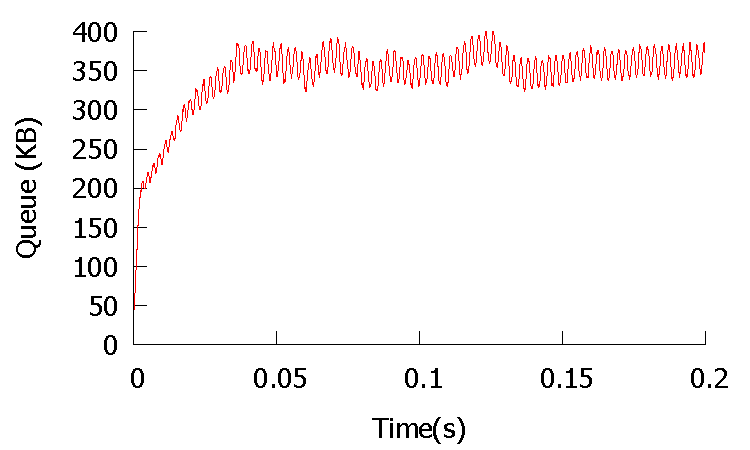
\includegraphics[width=0.3\textwidth]{figures/timely_stability_q_40f_fixed.pdf}
\label{fig:timely_fixed_c}
}
\vspace{-0.5em}
\caption{Performance of patched TIMELY}
\vspace{-0.5em}
\label{fig:timely_fixed}
\end{figure*}

In order to ensure there is a unique fixed point, and all flows get fair
share and are stable at the fixed point, we make two minor modifications over
TIMELY, as shown in Algorithm~\ref{fig:timely_fixed_algo}. We only modify the
last four lines of Algorithm~\ref{fig:timely_algo}.

\begin{algorithm}[t]
\footnotesize
{
\begin{algorithmic}[1]
%\Procedure{CalcRate}{$newRTT$}
\State $newRTTDiff \gets newRTT - prevRTT$
\State $prevRTT \gets newRTT$
\State $rttDiff \gets (1-\alpha) \cdot rttDiff + \alpha \cdot newRTTDiff$
\State $rttGradient = rttDiff/D_{minRTT}$
\If {$newRTT < T_{low}$}
        \State $rate \gets rate + \delta$
\ElsIf {$newRTT > T_{high}$}
        \State $rate \gets rate \cdot  (1 - \beta \cdot (1 - T_{high}/newRTT))$
\Else
		\State $weight \gets w(rttGradient)$	
		\State $error \gets \frac{{newRTT - RT{T_{ref}}}}{{RT{T_{ref}}}}$
        \State $rate \gets \delta (1-weight) +  rate \cdot (1 - \beta \cdot weight  \cdot error)$
\EndIf 
%\EndProcedure
\end{algorithmic}
}
\caption{Patched TIMELY rate calculation}
\label{fig:timely_fixed_algo}
\end{algorithm}

First, we make the step of rate decrease rely on absolute RTT, instead of the
gradient of RTT. In effect, this means that all flows have the knowledge of the
bottleneck queue length.  This ensures two things. First, the system can have a
unique fixed point, determined by the RTT\footnote{Recall that the issue with
the original TIMELY was that the RTT gradient could be the same, but absolute
RTTs could be different}.  Second, all flow can converge to the same rate, since
they share the knowledge of the bottleneck RTT.  The side effect, of course, is
that, with different number of flows, the fixed point of queue can be different.
We will address this in \S\ref{sec:discuss}. 

Second, we use a continuous weighting function $w(g)$ to make the transition
between rate increase and rate decrease smooth. This avoids the on-off behavior
that causes oscillation.  This is similar to the fact that probabilistic ECN
marking stabilizes TCP~\cite{misra2000fluid}, DCTCP~\cite{dctcp-analysis},
QCN~\cite{qcn-analysis} and DCQCN. With $w(g)$, we combine the two conditions of
$g \le 0$ and $g>0$ in the $dR(t)/dt$ equation:
\begin{equation}
\small
\frac{{dR_i}}{{dt}} = \left\{ \begin{array}{ll}
\frac{\delta }{{\tau *}}, & q(t - \tau ') < C*{T_{low}}\\
\frac{{(1 - {w_i})\delta }}{{\tau *}} - \frac{{{w_i}\beta {R_i}(t)}}{{\tau *}}\frac{{q(t - \tau ') - q'}}{{q'}}, & Otherwise\\
 - \frac{\beta }{{\tau *}}(1 - \frac{{C*{T_{high}}}}{{q(t - \tau ')}})R_i(t), & q(t - \tau ') > C*{T_{high}}
\end{array} \right.\\
\label{eq:timely_fixed}
\end{equation}
where $w_i$, the weight of rate decreasing, is a function of $g_i$, and must satisfy $0 \le w_i(g_i) \le 1$ for any $g$. 
Intuitively, $w_i(g_i)$ is monotonically increasing with $g_i$, because larger RTT gradient should lead to larger 
rate decrease. In original TIMELY protocol, $w_i(g_i)$ is an indicator function of $g_i$, {\em i.e.,} 
$w_i(g_i)=1$ when $g \le 0$, and $w_i(g_i)=0$ when $g<0$. Here we simply use a linear function of $g_i$ for $w_i$:
\begin{equation}
\small
{w_i} = \left\{ \begin{array}{ll}
0, & {g_i \le  - \frac{1}{4}} \\
2{g_i} + \frac{1}{2}, & { - \frac{1}{4} < g_i < \frac{1}{4}} \\
1, & {g_i \ge \frac{1}{4}}
\end{array} \right.
\end{equation}
In Equation~\ref{eq:timely_fixed}, $q'$ is a reference queue length. We simply set it as $C*T_{low}$, 
so that we decrease the rate faster if the queue length exceeds $C*T_{low}$. All
other TIMELY parameters remain the same except we set $\beta=0.008$ and $Seg=16KB$. 
We prove that this patched TIMELY protocol has desirable stability and convergence properties
that original TIMELY does not guarantee:


\begin{thm}[Patched TIMELY's fixed point.]
The system described in Equation~\ref{eq:timely_fixed} has a unique fixed point.
All flows have the same rate at this fixed point, and the queue length is:
\begin{equation}
\small
{q^*} = \frac{{N{R_{AI}}q'}}{{\beta C}} + q'
\label{eq:timely_fixed_q}
\end{equation}
The system described in Equation~\ref{eq:timely_fixed} always exponentially converges to 
the unique  fixed point.
\end{thm}

The detailed proof is omitted and can be found at~\cite{patchedtimelyproof}.



\if 0
\begin{proof}
Let the LHS of Equation~\ref{eq:timely_g} be 0, and $q(t - \tau ') - q(t - \tau ' - \tau *) = 0$ at the fixed 
point, we know $g_i^*=0$. Thus, $w_i^*=0.5$. Let the LHS of Equation~\ref{eq:timely_fixed} be 0. Because
all flows share the same queue length $q^*$, we have:
\begin{equation}
\small
R_1^* = R_2^* = ... = R_N^*
\end{equation}
The sum of all flow rates must be $C$ at the fixed point, therefore each flow has fair share $C/N$. 
\end{proof}
In addition, we can easily obtain the fixed point of queue length, which depends on $N$, the number of flows:
\begin{equation}
\small
{q^*} = \frac{{N{R_{AI}}q'}}{{\beta C}} + q'
\label{eq:timely_fixed_q}
\end{equation}

\begin{thm}[Patched TIMELY convergence.]
The system described in Equation~\ref{eq:timely_fixed} always converges to the unique fixed point.
\end{thm}
\begin{proof}
Here we provide a brief proof. First, the queue length $q$ always
converges to the fixed point $q^*$. This can be proved by contradiction because whenever $q$ stabilizes
at $q>q^*$, we have ${\left. {\frac{{dR}}{{dt}}} \right|_{q > {q^*}}} < {\left. {\frac{{dR}}{{dt}}} \right|_{q = {q^*}}} = 0$, 
leading to queue length decrease. The case of $q<q^*$ is similar. 

Second, once queue length converges to a stable state, we see that $g_i$ converges to 0.
We denote ${g_i}(n)$ as the value of $g_i$ upon the completion of $n$th segment after queue
length converges:
%Equation~\ref{eq:timely_g} becomes
%$\frac{{d{g_i}}}{{dt}} =  - \frac{\alpha }{{{\tau_i^*}}}{g_i}$. By turning it into a discrete model
%with $\tau_i^*(t)$ as intervals, we see that $g_i$ converges to 0:
\begin{equation}
\small
\left| {{g_i}(n + 1)} \right| = \left( {1 - \alpha} \right)\left| {{g_i}(n)} \right| = {\left( {1 - \alpha} \right)}^{n+1} \left| {{g_i}(0)} \right|
\end{equation}
Finally, after $g_i$ converges to 0, which means $w_i=0.5$, we rewrite the $j$th flow's Equation~\ref{eq:timely_fixed} 
and subtract it from $i$th flow's. Without losing generality, we choose $i,j, s.t.$ $i$th flow is the fastest among all flows,
whereas $j$th flow is the slowest. After simplification, we get:
\begin{equation}
\small
\frac{{d\left( {{R_i} - {R_j}} \right)}}{{dt}} = \frac{\delta }{{2Seg}}\left( {1 - \frac{N}{C}\left( {{R_i} + {R_j}} \right)} \right)\left( {{R_i} - {R_j}} \right)
\end{equation}
Among the total $N$ flows, there must exist at least one flow not slower than the fair share $C/N$.
Therefore, ${{R_i} + {R_j}} > C/N$ since $R_i$, the fastest flow, is not slower than $C/N$.
Solving the differential equation with ${{R_i} - {R_j}}$ as the variable, we get that the rate 
difference between the fastest and slowest flow decreases over time exponentially, as we shall see below. 

\para{Exponential convergence.} We estimate the TIMELY convergence time {\em after}
the queue stabilizes. We start from the case of $N=2$, where $R_i + R_j = C$
because of Equation~\ref{eq:timely_q}.
Then we get:
\begin{equation}
\small
{R_i}(t) - {R_j}(t) = \left( {{R_i}(0) - {R_j}(0)} \right){e^{\frac{{\delta (1 - N)}}{{2Seg}}t}}
\end{equation}
Once the fastest flow and slowest flow converge to the same rate, all flow rates converge to the unique fixed point.
\end{proof}

We use the same definition of ``converged'' as in
\S~\ref{sec:dcqcn_convergence}. Thus, the convergence
time is the smallest $t$ that satisfies (assuming two flows start with maximum possible rate difference, $C$):
\begin{equation}
\small
{e^{\frac{{\delta (1 - N)}}{{2Seg}}t}}C \le \frac{{0.1 \times C}}{N}
\label{eq:timely_convergence_time}
\end{equation}
With $N=2$ and parameters we choose earlier, we get $t = 76.7ms$. With (\ref{eq:timely_convergence_time}), 

It is easy to see that
with larger $N$,\footnote{Details omitted.} larger $\delta$ or smaller $Seg$, patched TIMELY will converge faster.

\fi

We verify patched TIMELY convergence and stability using simulations.
Figure~\ref{fig:timely_fixed_a} and~\ref{fig:timely_fixed_b}, shows that flows
with different initial rates converge to the fixed point and are stable without
oscillation, opposed to Figure~\ref{fig:ts2f73}. Results for the case depicted
in Figure~\ref{fig:ts2f55time} are similar.

\para{Stability.} We proceed as we did for DCQCN -- linearize the equations,
Laplace transform and compute the phase margin of its characteristic equation.
The phase margin result shows this system is stable until the number of flows is
greater than 40 (Figure~\ref{fig:timely_stability}).  This is again confirmed by
NS-3 simulation (Figure~\ref{fig:timely_fixed_b} and ~\ref{fig:timely_fixed_c}).
After 40 flows, the phase margin falls below 0 rapidly because more flows lead
to larger queue size (see Equation~\ref{eq:timely_fixed_q}), thus leading to
larger feedback delay (see Equation~\ref{eq:timely_taup}).  This leads to system
instability. In general, with some minor tuning, TIMELY can be stable within a
range of number of flows.
